%%%%%%%%%%%%%%%%%%%%%%%%%%%%%%%%%%%%%%%%%%%%%%%%%%%%%%%%%%%%%%%%%%%%%%%%%%%%%%%%%%%%%%%%%%%%%%%%%
%
% Document:      DM  product tree
%
%%%%%%%%%%%%%%%%%%%%%%%%%%%%%%%%%%%%%%%%%%%%%%%%%%%%%%%%%%%%%%%%%%%%%%%%%%%%%%
\documentclass{article}
\usepackage{times,layouts}
\usepackage{tikz,hyperref,amsmath}
\usetikzlibrary{positioning,arrows,shapes,decorations.shapes,shapes.arrows}
\usetikzlibrary{backgrounds,calc}
\usepackage[paperwidth=25cm,paperheight=150cm,
left=-2mm,top=3mm,bottom=0mm,right=0mm,
noheadfoot,marginparwidth=0pt,includemp=false,
textwidth=30cm,textheight=50mm]{geometry}
\newcommand\showpage{%
\setlayoutscale{0.5}\setlabelfont{\tiny}\printheadingsfalse\printparametersfalse
\currentpage\pagedesign}
\hypersetup{pdftitle={DM organisation }, pdfsubject={Diagram illustrating the
products in LSST DM }, pdfauthor={ William O'Mullane}}
\tikzstyle{wbbox}=[rectangle, rounded corners=3pt, draw=black, top color=blue!50!white, bottom color=white, very thick, minimum height=12mm, inner sep=2pt, text centered, text width=30mm] 
\tikzstyle{pbox}=[rectangle, rounded corners=3pt, draw=black, top color=yellow!50!white, bottom color=white, very thick, minimum height=7mm, inner sep=2pt, text centered, text width=35mm] 
\tikzstyle{pline}=[-, thick]\begin{document}
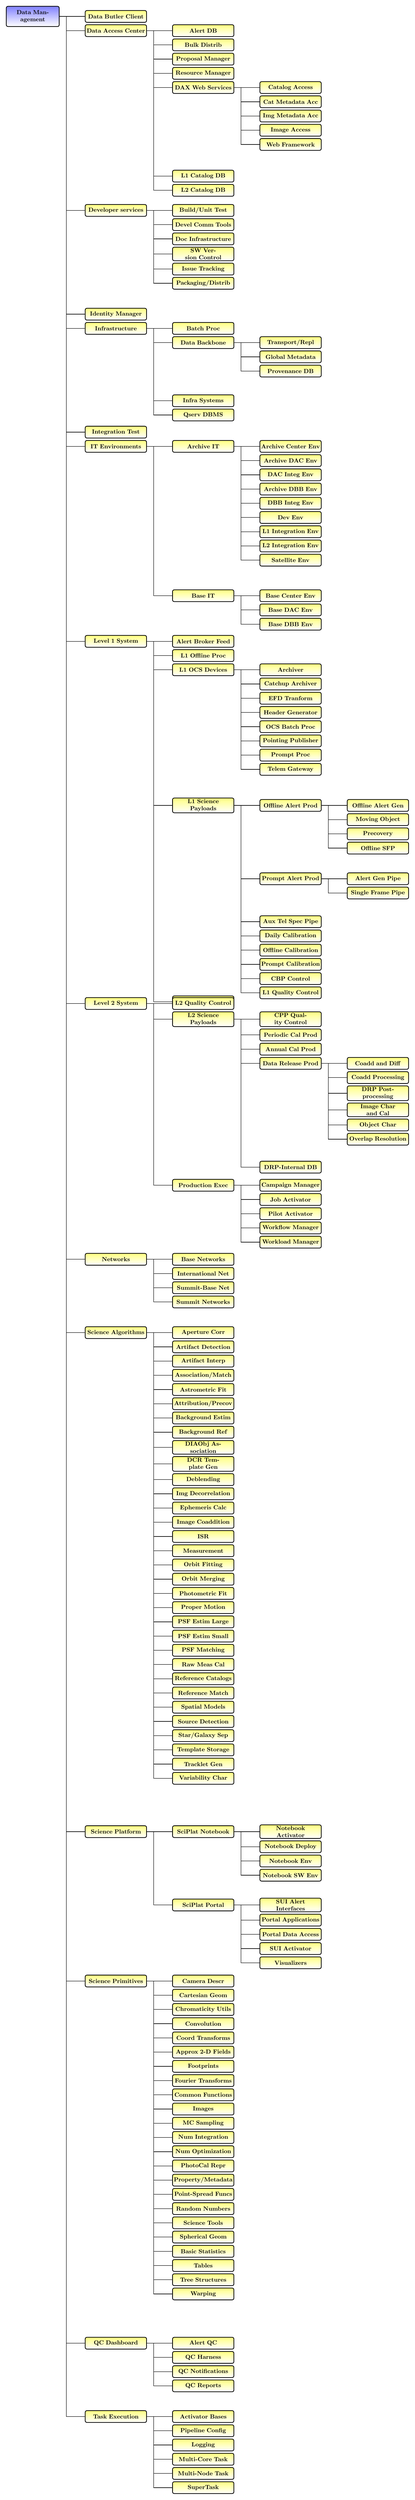
\begin{tikzpicture}[node distance=0mm]
\node (DM) [wbbox]{\textbf{Data Management}}; 
\node (BUTLER) [pbox,right=15mm of DM] {\textbf{Data Butler Client}}; 
 \draw[pline] (DM.east) -| ++(0.4,0)  |- (BUTLER.west);
 \node (DAC) [pbox,below=1mm of BUTLER] {\textbf{Data Access Center}}; 
 \draw[pline] (DM.east) -| ++(0.4,0)  |- (DAC.west);
 \node (ALERTDB) [pbox,right=15mm of DAC] {\textbf{Alert DB}}; 
 \draw[pline] (DAC.east) -| ++(0.4,0)  |- (ALERTDB.west);
 \node (BULKD) [pbox,below=1mm of ALERTDB] {\textbf{Bulk Distrib}}; 
 \draw[pline] (DAC.east) -| ++(0.4,0)  |- (BULKD.west);
 \node (DACPROP) [pbox,below=1mm of BULKD] {\textbf{Proposal Manager}}; 
 \draw[pline] (DAC.east) -| ++(0.4,0)  |- (DACPROP.west);
 \node (DACRM) [pbox,below=1mm of DACPROP] {\textbf{Resource Manager}}; 
 \draw[pline] (DAC.east) -| ++(0.4,0)  |- (DACRM.west);
 \node (DAX) [pbox,below=1mm of DACRM] {\textbf{DAX Web Services}}; 
 \draw[pline] (DAC.east) -| ++(0.4,0)  |- (DAX.west);
 \node (DAXCAT) [pbox,right=15mm of DAX] {\textbf{Catalog Access}}; 
 \draw[pline] (DAX.east) -| ++(0.4,0)  |- (DAXCAT.west);
 \node (DAXCMETA) [pbox,below=1mm of DAXCAT] {\textbf{Cat Metadata Acc}}; 
 \draw[pline] (DAX.east) -| ++(0.4,0)  |- (DAXCMETA.west);
 \node (DAXIMETA) [pbox,below=1mm of DAXCMETA] {\textbf{Img Metadata Acc}}; 
 \draw[pline] (DAX.east) -| ++(0.4,0)  |- (DAXIMETA.west);
 \node (DAXIMG) [pbox,below=1mm of DAXIMETA] {\textbf{Image Access}}; 
 \draw[pline] (DAX.east) -| ++(0.4,0)  |- (DAXIMG.west);
 \node (DAXWEB) [pbox,below=1mm of DAXIMG] {\textbf{Web Framework}}; 
 \draw[pline] (DAX.east) -| ++(0.4,0)  |- (DAXWEB.west);
 \node (L1DB) [pbox,below=45mm of DAX] {\textbf{L1 Catalog DB}}; 
 \draw[pline] (DAC.east) -| ++(0.4,0)  |- (L1DB.west);
 \node (L2DB) [pbox,below=1mm of L1DB] {\textbf{L2 Catalog DB}}; 
 \draw[pline] (DAC.east) -| ++(0.4,0)  |- (L2DB.west);
 \node (DEVEL) [pbox,below=99mm of DAC] {\textbf{Developer services}}; 
 \draw[pline] (DM.east) -| ++(0.4,0)  |- (DEVEL.west);
 \node (CI) [pbox,right=15mm of DEVEL] {\textbf{Build/Unit Test}}; 
 \draw[pline] (DEVEL.east) -| ++(0.4,0)  |- (CI.west);
 \node (COMMS) [pbox,below=1mm of CI] {\textbf{Devel Comm Tools}}; 
 \draw[pline] (DEVEL.east) -| ++(0.4,0)  |- (COMMS.west);
 \node (DOCS) [pbox,below=1mm of COMMS] {\textbf{Doc Infrastructure}}; 
 \draw[pline] (DEVEL.east) -| ++(0.4,0)  |- (DOCS.west);
 \node (DVCS) [pbox,below=1mm of DOCS] {\textbf{SW Version Control}}; 
 \draw[pline] (DEVEL.east) -| ++(0.4,0)  |- (DVCS.west);
 \node (ISSUE) [pbox,below=1mm of DVCS] {\textbf{Issue Tracking}}; 
 \draw[pline] (DEVEL.east) -| ++(0.4,0)  |- (ISSUE.west);
 \node (PKG) [pbox,below=1mm of ISSUE] {\textbf{Packaging/Distrib}}; 
 \draw[pline] (DEVEL.east) -| ++(0.4,0)  |- (PKG.west);
 \node (IDM) [pbox,below=54mm of DEVEL] {\textbf{Identity Manager}}; 
 \draw[pline] (DM.east) -| ++(0.4,0)  |- (IDM.west);
 \node (INFRA) [pbox,below=1mm of IDM] {\textbf{Infrastructure}}; 
 \draw[pline] (DM.east) -| ++(0.4,0)  |- (INFRA.west);
 \node (BPS) [pbox,right=15mm of INFRA] {\textbf{Batch Proc}}; 
 \draw[pline] (INFRA.east) -| ++(0.4,0)  |- (BPS.west);
 \node (DBB) [pbox,below=1mm of BPS] {\textbf{Data Backbone}}; 
 \draw[pline] (INFRA.east) -| ++(0.4,0)  |- (DBB.west);
 \node (DTR) [pbox,right=15mm of DBB] {\textbf{Transport/Repl}}; 
 \draw[pline] (DBB.east) -| ++(0.4,0)  |- (DTR.west);
 \node (GMDS) [pbox,below=1mm of DTR] {\textbf{Global Metadata}}; 
 \draw[pline] (DBB.east) -| ++(0.4,0)  |- (GMDS.west);
 \node (PRVDB) [pbox,below=1mm of GMDS] {\textbf{Provenance DB}}; 
 \draw[pline] (DBB.east) -| ++(0.4,0)  |- (PRVDB.west);
 \node (INFRASYS) [pbox,below=27mm of DBB] {\textbf{Infra Systems}}; 
 \draw[pline] (INFRA.east) -| ++(0.4,0)  |- (INFRASYS.west);
 \node (QSERV) [pbox,below=1mm of INFRASYS] {\textbf{Qserv DBMS}}; 
 \draw[pline] (INFRA.east) -| ++(0.4,0)  |- (QSERV.west);
 \node (INTGTEST) [pbox,below=54mm of INFRA] {\textbf{Integration Test}}; 
 \draw[pline] (DM.east) -| ++(0.4,0)  |- (INTGTEST.west);
 \node (ITENV) [pbox,below=1mm of INTGTEST] {\textbf{IT Environments}}; 
 \draw[pline] (DM.east) -| ++(0.4,0)  |- (ITENV.west);
 \node (ITARC) [pbox,right=15mm of ITENV] {\textbf{Archive IT}}; 
 \draw[pline] (ITENV.east) -| ++(0.4,0)  |- (ITARC.west);
 \node (CTRENV) [pbox,right=15mm of ITARC] {\textbf{Archive Center Env}}; 
 \draw[pline] (ITARC.east) -| ++(0.4,0)  |- (CTRENV.west);
 \node (DACENV) [pbox,below=1mm of CTRENV] {\textbf{Archive DAC Env}}; 
 \draw[pline] (ITARC.east) -| ++(0.4,0)  |- (DACENV.west);
 \node (DACINTGR) [pbox,below=1mm of DACENV] {\textbf{DAC Integ Env}}; 
 \draw[pline] (ITARC.east) -| ++(0.4,0)  |- (DACINTGR.west);
 \node (DBBENV) [pbox,below=1mm of DACINTGR] {\textbf{Archive DBB Env}}; 
 \draw[pline] (ITARC.east) -| ++(0.4,0)  |- (DBBENV.west);
 \node (DBBINTGR) [pbox,below=1mm of DBBENV] {\textbf{DBB Integ Env}}; 
 \draw[pline] (ITARC.east) -| ++(0.4,0)  |- (DBBINTGR.west);
 \node (DEVENV) [pbox,below=1mm of DBBINTGR] {\textbf{Dev Env}}; 
 \draw[pline] (ITARC.east) -| ++(0.4,0)  |- (DEVENV.west);
 \node (L1INTGR) [pbox,below=1mm of DEVENV] {\textbf{L1 Integration Env}}; 
 \draw[pline] (ITARC.east) -| ++(0.4,0)  |- (L1INTGR.west);
 \node (L2INTGR) [pbox,below=1mm of L1INTGR] {\textbf{L2 Integration Env}}; 
 \draw[pline] (ITARC.east) -| ++(0.4,0)  |- (L2INTGR.west);
 \node (SATENV) [pbox,below=1mm of L2INTGR] {\textbf{Satellite Env}}; 
 \draw[pline] (ITARC.east) -| ++(0.4,0)  |- (SATENV.west);
 \node (ITBASE) [pbox,below=81mm of ITARC] {\textbf{Base IT}}; 
 \draw[pline] (ITENV.east) -| ++(0.4,0)  |- (ITBASE.west);
 \node (BCTRENV) [pbox,right=15mm of ITBASE] {\textbf{Base Center Env}}; 
 \draw[pline] (ITBASE.east) -| ++(0.4,0)  |- (BCTRENV.west);
 \node (BDACENV) [pbox,below=1mm of BCTRENV] {\textbf{Base DAC Env}}; 
 \draw[pline] (ITBASE.east) -| ++(0.4,0)  |- (BDACENV.west);
 \node (BDBBENV) [pbox,below=1mm of BDACENV] {\textbf{Base DBB Env}}; 
 \draw[pline] (ITBASE.east) -| ++(0.4,0)  |- (BDBBENV.west);
 \node (L1) [pbox,below=108mm of ITENV] {\textbf{Level 1 System}}; 
 \draw[pline] (DM.east) -| ++(0.4,0)  |- (L1.west);
 \node (BRKRFEED) [pbox,right=15mm of L1] {\textbf{Alert Broker Feed}}; 
 \draw[pline] (L1.east) -| ++(0.4,0)  |- (BRKRFEED.west);
 \node (L1OFFL) [pbox,below=1mm of BRKRFEED] {\textbf{L1 Offline Proc}}; 
 \draw[pline] (L1.east) -| ++(0.4,0)  |- (L1OFFL.west);
 \node (L1ONL) [pbox,below=1mm of L1OFFL] {\textbf{L1 OCS Devices}}; 
 \draw[pline] (L1.east) -| ++(0.4,0)  |- (L1ONL.west);
 \node (ARC) [pbox,right=15mm of L1ONL] {\textbf{Archiver}}; 
 \draw[pline] (L1ONL.east) -| ++(0.4,0)  |- (ARC.west);
 \node (CARC) [pbox,below=1mm of ARC] {\textbf{Catchup Archiver}}; 
 \draw[pline] (L1ONL.east) -| ++(0.4,0)  |- (CARC.west);
 \node (EFDT) [pbox,below=1mm of CARC] {\textbf{EFD Tranform}}; 
 \draw[pline] (L1ONL.east) -| ++(0.4,0)  |- (EFDT.west);
 \node (HEADER) [pbox,below=1mm of EFDT] {\textbf{Header Generator}}; 
 \draw[pline] (L1ONL.east) -| ++(0.4,0)  |- (HEADER.west);
 \node (OCSBAT) [pbox,below=1mm of HEADER] {\textbf{OCS Batch Proc}}; 
 \draw[pline] (L1ONL.east) -| ++(0.4,0)  |- (OCSBAT.west);
 \node (POINTP) [pbox,below=1mm of OCSBAT] {\textbf{Pointing Publisher}}; 
 \draw[pline] (L1ONL.east) -| ++(0.4,0)  |- (POINTP.west);
 \node (PRMPT) [pbox,below=1mm of POINTP] {\textbf{Prompt Proc}}; 
 \draw[pline] (L1ONL.east) -| ++(0.4,0)  |- (PRMPT.west);
 \node (TMG) [pbox,below=1mm of PRMPT] {\textbf{Telem Gateway}}; 
 \draw[pline] (L1ONL.east) -| ++(0.4,0)  |- (TMG.west);
 \node (L1SCI) [pbox,below=72mm of L1ONL] {\textbf{L1 Science Payloads}}; 
 \draw[pline] (L1.east) -| ++(0.4,0)  |- (L1SCI.west);
 \node (APOFFL) [pbox,right=15mm of L1SCI] {\textbf{Offline Alert Prod}}; 
 \draw[pline] (L1SCI.east) -| ++(0.4,0)  |- (APOFFL.west);
 \node (ALRTOFFL) [pbox,right=15mm of APOFFL] {\textbf{Offline Alert Gen}}; 
 \draw[pline] (APOFFL.east) -| ++(0.4,0)  |- (ALRTOFFL.west);
 \node (MOPS) [pbox,below=1mm of ALRTOFFL] {\textbf{Moving Object}}; 
 \draw[pline] (APOFFL.east) -| ++(0.4,0)  |- (MOPS.west);
 \node (PRECOV) [pbox,below=1mm of MOPS] {\textbf{Precovery}}; 
 \draw[pline] (APOFFL.east) -| ++(0.4,0)  |- (PRECOV.west);
 \node (SFPOFFL) [pbox,below=1mm of PRECOV] {\textbf{Offline SFP}}; 
 \draw[pline] (APOFFL.east) -| ++(0.4,0)  |- (SFPOFFL.west);
 \node (APPRMPT) [pbox,below=36mm of APOFFL] {\textbf{Prompt Alert Prod}}; 
 \draw[pline] (L1SCI.east) -| ++(0.4,0)  |- (APPRMPT.west);
 \node (ALERTPIPE) [pbox,right=15mm of APPRMPT] {\textbf{Alert Gen Pipe}}; 
 \draw[pline] (APPRMPT.east) -| ++(0.4,0)  |- (ALERTPIPE.west);
 \node (SFPPIPE) [pbox,below=1mm of ALERTPIPE] {\textbf{Single Frame Pipe}}; 
 \draw[pline] (APPRMPT.east) -| ++(0.4,0)  |- (SFPPIPE.west);
 \node (AUXTEL) [pbox,below=18mm of APPRMPT] {\textbf{Aux Tel Spec Pipe}}; 
 \draw[pline] (L1SCI.east) -| ++(0.4,0)  |- (AUXTEL.west);
 \node (CALDAILY) [pbox,below=1mm of AUXTEL] {\textbf{Daily Calibration}}; 
 \draw[pline] (L1SCI.east) -| ++(0.4,0)  |- (CALDAILY.west);
 \node (CALOFFL) [pbox,below=1mm of CALDAILY] {\textbf{Offline Calibration}}; 
 \draw[pline] (L1SCI.east) -| ++(0.4,0)  |- (CALOFFL.west);
 \node (CALPRMPT) [pbox,below=1mm of CALOFFL] {\textbf{Prompt Calibration}}; 
 \draw[pline] (L1SCI.east) -| ++(0.4,0)  |- (CALPRMPT.west);
 \node (CBPCTRL) [pbox,below=1mm of CALPRMPT] {\textbf{CBP Control}}; 
 \draw[pline] (L1SCI.east) -| ++(0.4,0)  |- (CBPCTRL.west);
 \node (L1QC) [pbox,below=1mm of CBPCTRL] {\textbf{L1 Quality Control}}; 
 \draw[pline] (L1SCI.east) -| ++(0.4,0)  |- (L1QC.west);
 \node (MINIBRKR) [pbox,below=108mm of L1SCI] {\textbf{Alert Mini-Broker}}; 
 \draw[pline] (L1.east) -| ++(0.4,0)  |- (MINIBRKR.west);
 \node (L2) [pbox,below=207mm of L1] {\textbf{Level 2 System}}; 
 \draw[pline] (DM.east) -| ++(0.4,0)  |- (L2.west);
 \node (L2QC) [pbox,right=15mm of L2] {\textbf{L2 Quality Control}}; 
 \draw[pline] (L2.east) -| ++(0.4,0)  |- (L2QC.west);
 \node (L2SCI) [pbox,below=1mm of L2QC] {\textbf{L2 Science Payloads}}; 
 \draw[pline] (L2.east) -| ++(0.4,0)  |- (L2SCI.west);
 \node (CPPQC) [pbox,right=15mm of L2SCI] {\textbf{CPP Quality Control}}; 
 \draw[pline] (L2SCI.east) -| ++(0.4,0)  |- (CPPQC.west);
 \node (CPPSLOW) [pbox,below=1mm of CPPQC] {\textbf{Periodic Cal Prod}}; 
 \draw[pline] (L2SCI.east) -| ++(0.4,0)  |- (CPPSLOW.west);
 \node (CPPYEAR) [pbox,below=1mm of CPPSLOW] {\textbf{Annual Cal Prod}}; 
 \draw[pline] (L2SCI.east) -| ++(0.4,0)  |- (CPPYEAR.west);
 \node (DRP) [pbox,below=1mm of CPPYEAR] {\textbf{Data Release Prod}}; 
 \draw[pline] (L2SCI.east) -| ++(0.4,0)  |- (DRP.west);
 \node (COADPIPE) [pbox,right=15mm of DRP] {\textbf{Coadd and Diff}}; 
 \draw[pline] (DRP.east) -| ++(0.4,0)  |- (COADPIPE.west);
 \node (COADPROC) [pbox,below=1mm of COADPIPE] {\textbf{Coadd Processing}}; 
 \draw[pline] (DRP.east) -| ++(0.4,0)  |- (COADPROC.west);
 \node (DRPPOST) [pbox,below=1mm of COADPROC] {\textbf{DRP Postprocessing}}; 
 \draw[pline] (DRP.east) -| ++(0.4,0)  |- (DRPPOST.west);
 \node (IMGCHAR) [pbox,below=1mm of DRPPOST] {\textbf{Image Char and Cal}}; 
 \draw[pline] (DRP.east) -| ++(0.4,0)  |- (IMGCHAR.west);
 \node (MULTIFIT) [pbox,below=1mm of IMGCHAR] {\textbf{Object Char}}; 
 \draw[pline] (DRP.east) -| ++(0.4,0)  |- (MULTIFIT.west);
 \node (OVERLAP) [pbox,below=1mm of MULTIFIT] {\textbf{Overlap Resolution}}; 
 \draw[pline] (DRP.east) -| ++(0.4,0)  |- (OVERLAP.west);
 \node (DRPDB) [pbox,below=54mm of DRP] {\textbf{DRP-Internal DB}}; 
 \draw[pline] (L2SCI.east) -| ++(0.4,0)  |- (DRPDB.west);
 \node (PRODEX) [pbox,below=90mm of L2SCI] {\textbf{Production Exec}}; 
 \draw[pline] (L2.east) -| ++(0.4,0)  |- (PRODEX.west);
 \node (CMPGN) [pbox,right=15mm of PRODEX] {\textbf{Campaign Manager}}; 
 \draw[pline] (PRODEX.east) -| ++(0.4,0)  |- (CMPGN.west);
 \node (JOBACTIV) [pbox,below=1mm of CMPGN] {\textbf{Job Activator}}; 
 \draw[pline] (PRODEX.east) -| ++(0.4,0)  |- (JOBACTIV.west);
 \node (PLTACTIV) [pbox,below=1mm of JOBACTIV] {\textbf{Pilot Activator}}; 
 \draw[pline] (PRODEX.east) -| ++(0.4,0)  |- (PLTACTIV.west);
 \node (WFM) [pbox,below=1mm of PLTACTIV] {\textbf{Workflow Manager}}; 
 \draw[pline] (PRODEX.east) -| ++(0.4,0)  |- (WFM.west);
 \node (WLM) [pbox,below=1mm of WFM] {\textbf{Workload Manager}}; 
 \draw[pline] (PRODEX.east) -| ++(0.4,0)  |- (WLM.west);
 \node (NET) [pbox,below=144mm of L2] {\textbf{Networks}}; 
 \draw[pline] (DM.east) -| ++(0.4,0)  |- (NET.west);
 \node (NETBASE) [pbox,right=15mm of NET] {\textbf{Base Networks}}; 
 \draw[pline] (NET.east) -| ++(0.4,0)  |- (NETBASE.west);
 \node (NETINTL) [pbox,below=1mm of NETBASE] {\textbf{International Net}}; 
 \draw[pline] (NET.east) -| ++(0.4,0)  |- (NETINTL.west);
 \node (NETSB) [pbox,below=1mm of NETINTL] {\textbf{Summit-Base Net}}; 
 \draw[pline] (NET.east) -| ++(0.4,0)  |- (NETSB.west);
 \node (NETSUM) [pbox,below=1mm of NETSB] {\textbf{Summit Networks}}; 
 \draw[pline] (NET.east) -| ++(0.4,0)  |- (NETSUM.west);
 \node (SCIALG) [pbox,below=36mm of NET] {\textbf{Science Algorithms}}; 
 \draw[pline] (DM.east) -| ++(0.4,0)  |- (SCIALG.west);
 \node (APCORR) [pbox,right=15mm of SCIALG] {\textbf{Aperture Corr}}; 
 \draw[pline] (SCIALG.east) -| ++(0.4,0)  |- (APCORR.west);
 \node (ARTFDET) [pbox,below=1mm of APCORR] {\textbf{Artifact Detection}}; 
 \draw[pline] (SCIALG.east) -| ++(0.4,0)  |- (ARTFDET.west);
 \node (ARTFINTP) [pbox,below=1mm of ARTFDET] {\textbf{Artifact Interp}}; 
 \draw[pline] (SCIALG.east) -| ++(0.4,0)  |- (ARTFINTP.west);
 \node (ASSOC) [pbox,below=1mm of ARTFINTP] {\textbf{Association/Match}}; 
 \draw[pline] (SCIALG.east) -| ++(0.4,0)  |- (ASSOC.west);
 \node (ASTROM) [pbox,below=1mm of ASSOC] {\textbf{Astrometric Fit}}; 
 \draw[pline] (SCIALG.east) -| ++(0.4,0)  |- (ASTROM.west);
 \node (ATTRIB) [pbox,below=1mm of ASTROM] {\textbf{Attribution/Precov}}; 
 \draw[pline] (SCIALG.east) -| ++(0.4,0)  |- (ATTRIB.west);
 \node (BKGDEST) [pbox,below=1mm of ATTRIB] {\textbf{Background Estim}}; 
 \draw[pline] (SCIALG.east) -| ++(0.4,0)  |- (BKGDEST.west);
 \node (BKGDREF) [pbox,below=1mm of BKGDEST] {\textbf{Background Ref}}; 
 \draw[pline] (SCIALG.east) -| ++(0.4,0)  |- (BKGDREF.west);
 \node (DASSOC) [pbox,below=1mm of BKGDREF] {\textbf{DIAObj Association}}; 
 \draw[pline] (SCIALG.east) -| ++(0.4,0)  |- (DASSOC.west);
 \node (DCRTMPL) [pbox,below=1mm of DASSOC] {\textbf{DCR Template Gen}}; 
 \draw[pline] (SCIALG.east) -| ++(0.4,0)  |- (DCRTMPL.west);
 \node (DEBLEND) [pbox,below=1mm of DCRTMPL] {\textbf{Deblending}}; 
 \draw[pline] (SCIALG.east) -| ++(0.4,0)  |- (DEBLEND.west);
 \node (DECORR) [pbox,below=1mm of DEBLEND] {\textbf{Img Decorrelation}}; 
 \draw[pline] (SCIALG.east) -| ++(0.4,0)  |- (DECORR.west);
 \node (EPHEM) [pbox,below=1mm of DECORR] {\textbf{Ephemeris Calc}}; 
 \draw[pline] (SCIALG.east) -| ++(0.4,0)  |- (EPHEM.west);
 \node (IMCOADD) [pbox,below=1mm of EPHEM] {\textbf{Image Coaddition}}; 
 \draw[pline] (SCIALG.east) -| ++(0.4,0)  |- (IMCOADD.west);
 \node (ISR) [pbox,below=1mm of IMCOADD] {\textbf{ISR}}; 
 \draw[pline] (SCIALG.east) -| ++(0.4,0)  |- (ISR.west);
 \node (MEASURE) [pbox,below=1mm of ISR] {\textbf{Measurement}}; 
 \draw[pline] (SCIALG.east) -| ++(0.4,0)  |- (MEASURE.west);
 \node (ORBFIT) [pbox,below=1mm of MEASURE] {\textbf{Orbit Fitting}}; 
 \draw[pline] (SCIALG.east) -| ++(0.4,0)  |- (ORBFIT.west);
 \node (ORBMERGE) [pbox,below=1mm of ORBFIT] {\textbf{Orbit Merging}}; 
 \draw[pline] (SCIALG.east) -| ++(0.4,0)  |- (ORBMERGE.west);
 \node (PHOTOM) [pbox,below=1mm of ORBMERGE] {\textbf{Photometric Fit}}; 
 \draw[pline] (SCIALG.east) -| ++(0.4,0)  |- (PHOTOM.west);
 \node (PRPRMOT) [pbox,below=1mm of PHOTOM] {\textbf{Proper Motion}}; 
 \draw[pline] (SCIALG.east) -| ++(0.4,0)  |- (PRPRMOT.west);
 \node (PSFESTLG) [pbox,below=1mm of PRPRMOT] {\textbf{PSF Estim Large}}; 
 \draw[pline] (SCIALG.east) -| ++(0.4,0)  |- (PSFESTLG.west);
 \node (PSFESTSM) [pbox,below=1mm of PSFESTLG] {\textbf{PSF Estim Small}}; 
 \draw[pline] (SCIALG.east) -| ++(0.4,0)  |- (PSFESTSM.west);
 \node (PSFMATCH) [pbox,below=1mm of PSFESTSM] {\textbf{PSF Matching}}; 
 \draw[pline] (SCIALG.east) -| ++(0.4,0)  |- (PSFMATCH.west);
 \node (RAWCAL) [pbox,below=1mm of PSFMATCH] {\textbf{Raw Meas Cal}}; 
 \draw[pline] (SCIALG.east) -| ++(0.4,0)  |- (RAWCAL.west);
 \node (REFCAT) [pbox,below=1mm of RAWCAL] {\textbf{Reference Catalogs}}; 
 \draw[pline] (SCIALG.east) -| ++(0.4,0)  |- (REFCAT.west);
 \node (REFMATCH) [pbox,below=1mm of REFCAT] {\textbf{Reference Match}}; 
 \draw[pline] (SCIALG.east) -| ++(0.4,0)  |- (REFMATCH.west);
 \node (SPATMOD) [pbox,below=1mm of REFMATCH] {\textbf{Spatial Models}}; 
 \draw[pline] (SCIALG.east) -| ++(0.4,0)  |- (SPATMOD.west);
 \node (SRCDET) [pbox,below=1mm of SPATMOD] {\textbf{Source Detection}}; 
 \draw[pline] (SCIALG.east) -| ++(0.4,0)  |- (SRCDET.west);
 \node (STARGAL) [pbox,below=1mm of SRCDET] {\textbf{Star/Galaxy Sep}}; 
 \draw[pline] (SCIALG.east) -| ++(0.4,0)  |- (STARGAL.west);
 \node (TEMPLATE) [pbox,below=1mm of STARGAL] {\textbf{Template Storage}}; 
 \draw[pline] (SCIALG.east) -| ++(0.4,0)  |- (TEMPLATE.west);
 \node (TRACKLET) [pbox,below=1mm of TEMPLATE] {\textbf{Tracklet Gen}}; 
 \draw[pline] (SCIALG.east) -| ++(0.4,0)  |- (TRACKLET.west);
 \node (VRBLTY) [pbox,below=1mm of TRACKLET] {\textbf{Variability Char}}; 
 \draw[pline] (SCIALG.east) -| ++(0.4,0)  |- (VRBLTY.west);
 \node (SCIPLAT) [pbox,below=288mm of SCIALG] {\textbf{Science Platform}}; 
 \draw[pline] (DM.east) -| ++(0.4,0)  |- (SCIPLAT.west);
 \node (SPLNBK) [pbox,right=15mm of SCIPLAT] {\textbf{SciPlat Notebook}}; 
 \draw[pline] (SCIPLAT.east) -| ++(0.4,0)  |- (SPLNBK.west);
 \node (NBKACTIV) [pbox,right=15mm of SPLNBK] {\textbf{Notebook Activator}}; 
 \draw[pline] (SPLNBK.east) -| ++(0.4,0)  |- (NBKACTIV.west);
 \node (NBKDPLY) [pbox,below=1mm of NBKACTIV] {\textbf{Notebook Deploy}}; 
 \draw[pline] (SPLNBK.east) -| ++(0.4,0)  |- (NBKDPLY.west);
 \node (NBKENV) [pbox,below=1mm of NBKDPLY] {\textbf{Notebook Env}}; 
 \draw[pline] (SPLNBK.east) -| ++(0.4,0)  |- (NBKENV.west);
 \node (NBKSW) [pbox,below=1mm of NBKENV] {\textbf{Notebook SW Env}}; 
 \draw[pline] (SPLNBK.east) -| ++(0.4,0)  |- (NBKSW.west);
 \node (SPLPRTL) [pbox,below=36mm of SPLNBK] {\textbf{SciPlat Portal}}; 
 \draw[pline] (SCIPLAT.east) -| ++(0.4,0)  |- (SPLPRTL.west);
 \node (PRTLALRT) [pbox,right=15mm of SPLPRTL] {\textbf{SUI Alert Interfaces}}; 
 \draw[pline] (SPLPRTL.east) -| ++(0.4,0)  |- (PRTLALRT.west);
 \node (PRTLAPPS) [pbox,below=1mm of PRTLALRT] {\textbf{Portal Applications}}; 
 \draw[pline] (SPLPRTL.east) -| ++(0.4,0)  |- (PRTLAPPS.west);
 \node (PRTLDAX) [pbox,below=1mm of PRTLAPPS] {\textbf{Portal Data Access}}; 
 \draw[pline] (SPLPRTL.east) -| ++(0.4,0)  |- (PRTLDAX.west);
 \node (SUIACTIV) [pbox,below=1mm of PRTLDAX] {\textbf{SUI Activator}}; 
 \draw[pline] (SPLPRTL.east) -| ++(0.4,0)  |- (SUIACTIV.west);
 \node (VIS) [pbox,below=1mm of SUIACTIV] {\textbf{Visualizers}}; 
 \draw[pline] (SPLPRTL.east) -| ++(0.4,0)  |- (VIS.west);
 \node (SCIPRIM) [pbox,below=81mm of SCIPLAT] {\textbf{Science Primitives}}; 
 \draw[pline] (DM.east) -| ++(0.4,0)  |- (SCIPRIM.west);
 \node (CAMDESC) [pbox,right=15mm of SCIPRIM] {\textbf{Camera Descr}}; 
 \draw[pline] (SCIPRIM.east) -| ++(0.4,0)  |- (CAMDESC.west);
 \node (CARTGEOM) [pbox,below=1mm of CAMDESC] {\textbf{Cartesian Geom}}; 
 \draw[pline] (SCIPRIM.east) -| ++(0.4,0)  |- (CARTGEOM.west);
 \node (CHROM) [pbox,below=1mm of CARTGEOM] {\textbf{Chromaticity Utils}}; 
 \draw[pline] (SCIPRIM.east) -| ++(0.4,0)  |- (CHROM.west);
 \node (CONVOL) [pbox,below=1mm of CHROM] {\textbf{Convolution}}; 
 \draw[pline] (SCIPRIM.east) -| ++(0.4,0)  |- (CONVOL.west);
 \node (COORD) [pbox,below=1mm of CONVOL] {\textbf{Coord Transforms}}; 
 \draw[pline] (SCIPRIM.east) -| ++(0.4,0)  |- (COORD.west);
 \node (FIELDS) [pbox,below=1mm of COORD] {\textbf{Approx 2-D Fields}}; 
 \draw[pline] (SCIPRIM.east) -| ++(0.4,0)  |- (FIELDS.west);
 \node (FOOTPRNT) [pbox,below=1mm of FIELDS] {\textbf{Footprints}}; 
 \draw[pline] (SCIPRIM.east) -| ++(0.4,0)  |- (FOOTPRNT.west);
 \node (FT) [pbox,below=1mm of FOOTPRNT] {\textbf{Fourier Transforms}}; 
 \draw[pline] (SCIPRIM.east) -| ++(0.4,0)  |- (FT.west);
 \node (FUNCTION) [pbox,below=1mm of FT] {\textbf{Common Functions}}; 
 \draw[pline] (SCIPRIM.east) -| ++(0.4,0)  |- (FUNCTION.west);
 \node (IMAGE) [pbox,below=1mm of FUNCTION] {\textbf{Images}}; 
 \draw[pline] (SCIPRIM.east) -| ++(0.4,0)  |- (IMAGE.west);
 \node (MCSAMP) [pbox,below=1mm of IMAGE] {\textbf{MC Sampling}}; 
 \draw[pline] (SCIPRIM.east) -| ++(0.4,0)  |- (MCSAMP.west);
 \node (NUMINTEG) [pbox,below=1mm of MCSAMP] {\textbf{Num Integration}}; 
 \draw[pline] (SCIPRIM.east) -| ++(0.4,0)  |- (NUMINTEG.west);
 \node (NUMOPTIM) [pbox,below=1mm of NUMINTEG] {\textbf{Num Optimization}}; 
 \draw[pline] (SCIPRIM.east) -| ++(0.4,0)  |- (NUMOPTIM.west);
 \node (PHOTPRIM) [pbox,below=1mm of NUMOPTIM] {\textbf{PhotoCal Repr}}; 
 \draw[pline] (SCIPRIM.east) -| ++(0.4,0)  |- (PHOTPRIM.west);
 \node (PROPSET) [pbox,below=1mm of PHOTPRIM] {\textbf{Property/Metadata}}; 
 \draw[pline] (SCIPRIM.east) -| ++(0.4,0)  |- (PROPSET.west);
 \node (PSF) [pbox,below=1mm of PROPSET] {\textbf{Point-Spread Funcs}}; 
 \draw[pline] (SCIPRIM.east) -| ++(0.4,0)  |- (PSF.west);
 \node (RANDOM) [pbox,below=1mm of PSF] {\textbf{Random Numbers}}; 
 \draw[pline] (SCIPRIM.east) -| ++(0.4,0)  |- (RANDOM.west);
 \node (SCITOOLS) [pbox,below=1mm of RANDOM] {\textbf{Science Tools}}; 
 \draw[pline] (SCIPRIM.east) -| ++(0.4,0)  |- (SCITOOLS.west);
 \node (SPHGEOM) [pbox,below=1mm of SCITOOLS] {\textbf{Spherical Geom}}; 
 \draw[pline] (SCIPRIM.east) -| ++(0.4,0)  |- (SPHGEOM.west);
 \node (STATS) [pbox,below=1mm of SPHGEOM] {\textbf{Basic Statistics}}; 
 \draw[pline] (SCIPRIM.east) -| ++(0.4,0)  |- (STATS.west);
 \node (TABLE) [pbox,below=1mm of STATS] {\textbf{Tables}}; 
 \draw[pline] (SCIPRIM.east) -| ++(0.4,0)  |- (TABLE.west);
 \node (TREES) [pbox,below=1mm of TABLE] {\textbf{Tree Structures}}; 
 \draw[pline] (SCIPRIM.east) -| ++(0.4,0)  |- (TREES.west);
 \node (WARP) [pbox,below=1mm of TREES] {\textbf{Warping}}; 
 \draw[pline] (SCIPRIM.east) -| ++(0.4,0)  |- (WARP.west);
 \node (SQUASH) [pbox,below=207mm of SCIPRIM] {\textbf{QC Dashboard}}; 
 \draw[pline] (DM.east) -| ++(0.4,0)  |- (SQUASH.west);
 \node (SQALERT) [pbox,right=15mm of SQUASH] {\textbf{Alert QC}}; 
 \draw[pline] (SQUASH.east) -| ++(0.4,0)  |- (SQALERT.west);
 \node (SQHARN) [pbox,below=1mm of SQALERT] {\textbf{QC Harness}}; 
 \draw[pline] (SQUASH.east) -| ++(0.4,0)  |- (SQHARN.west);
 \node (SQNOTIF) [pbox,below=1mm of SQHARN] {\textbf{QC Notifications}}; 
 \draw[pline] (SQUASH.east) -| ++(0.4,0)  |- (SQNOTIF.west);
 \node (SQREPORT) [pbox,below=1mm of SQNOTIF] {\textbf{QC Reports}}; 
 \draw[pline] (SQUASH.east) -| ++(0.4,0)  |- (SQREPORT.west);
 \node (TXF) [pbox,below=36mm of SQUASH] {\textbf{Task Execution}}; 
 \draw[pline] (DM.east) -| ++(0.4,0)  |- (TXF.west);
 \node (ACTIVATR) [pbox,right=15mm of TXF] {\textbf{Activator Bases}}; 
 \draw[pline] (TXF.east) -| ++(0.4,0)  |- (ACTIVATR.west);
 \node (CONFIG) [pbox,below=1mm of ACTIVATR] {\textbf{Pipeline Config}}; 
 \draw[pline] (TXF.east) -| ++(0.4,0)  |- (CONFIG.west);
 \node (LOG) [pbox,below=1mm of CONFIG] {\textbf{Logging}}; 
 \draw[pline] (TXF.east) -| ++(0.4,0)  |- (LOG.west);
 \node (MULTCORE) [pbox,below=1mm of LOG] {\textbf{Multi-Core Task}}; 
 \draw[pline] (TXF.east) -| ++(0.4,0)  |- (MULTCORE.west);
 \node (MULTNODE) [pbox,below=1mm of MULTCORE] {\textbf{Multi-Node Task}}; 
 \draw[pline] (TXF.east) -| ++(0.4,0)  |- (MULTNODE.west);
 \node (SPRTASK) [pbox,below=1mm of MULTNODE] {\textbf{SuperTask}}; 
 \draw[pline] (TXF.east) -| ++(0.4,0)  |- (SPRTASK.west);
 \end{tikzpicture}
\end{document}
